\documentclass{article}
\usepackage[utf8]{inputenc}
\usepackage{tikz}
\usetikzlibrary{positioning}
\usetikzlibrary{shapes}

\begin{document}

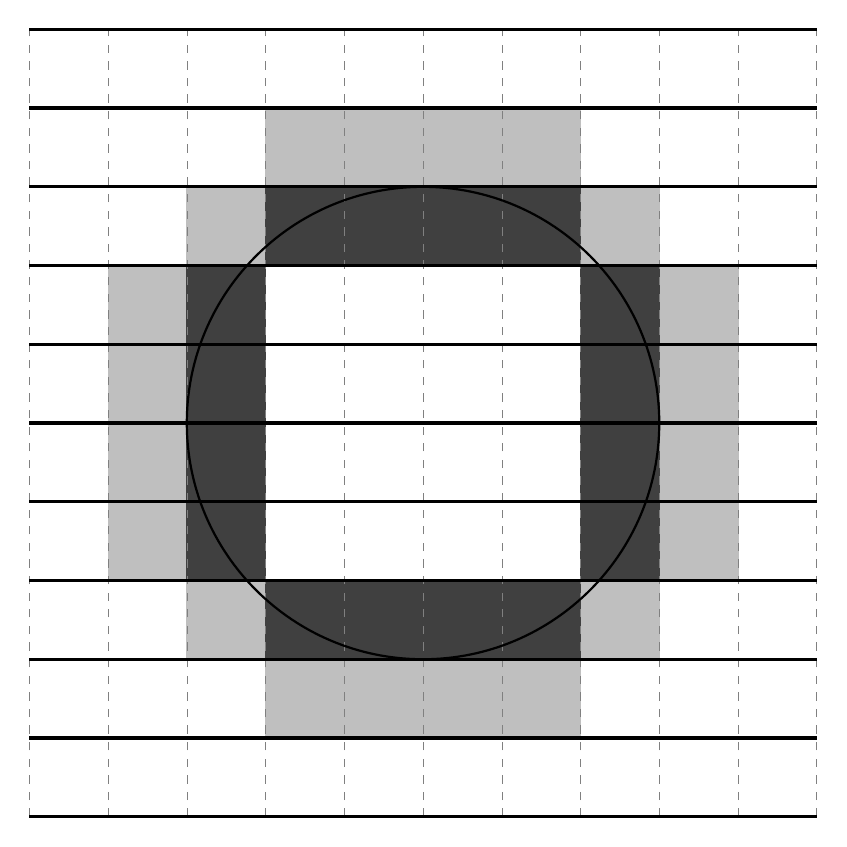
\begin{tikzpicture}
%shaded squares
\filldraw[lightgray] ([xshift=-0.5cm,yshift=-0.5cm]	4.5,1.5) rectangle ++(1cm,1cm);
\filldraw[lightgray] ([xshift=-0.5cm,yshift=-0.5cm]	3.5,1.5) rectangle ++(1cm,1cm);
\filldraw[lightgray] ([xshift=-0.5cm,yshift=-0.5cm]	2.5,2.5) rectangle ++(1cm,1cm);
\filldraw[lightgray] ([xshift=-0.5cm,yshift=-0.5cm]	1.5,3.5) rectangle ++(1cm,1cm);
\filldraw[lightgray] ([xshift=-0.5cm,yshift=-0.5cm]	1.5,4.5) rectangle ++(1cm,1cm);
\filldraw[lightgray] ([xshift=-0.5cm,yshift=-0.5cm]	4.5,8.5) rectangle ++(1cm,1cm);
\filldraw[lightgray] ([xshift=-0.5cm,yshift=-0.5cm]	3.5,8.5) rectangle ++(1cm,1cm);
\filldraw[lightgray] ([xshift=-0.5cm,yshift=-0.5cm]	2.5,7.5) rectangle ++(1cm,1cm);
\filldraw[lightgray] ([xshift=-0.5cm,yshift=-0.5cm]	1.5,6.5) rectangle ++(1cm,1cm);
\filldraw[lightgray] ([xshift=-0.5cm,yshift=-0.5cm]	1.5,5.5) rectangle ++(1cm,1cm);

\filldraw[lightgray] ([xshift=-0.5cm,yshift=-0.5cm]	5.5,1.5) rectangle ++(1cm,1cm);
\filldraw[lightgray] ([xshift=-0.5cm,yshift=-0.5cm]	6.5,1.5) rectangle ++(1cm,1cm);
\filldraw[lightgray] ([xshift=-0.5cm,yshift=-0.5cm]	7.5,2.5) rectangle ++(1cm,1cm);
\filldraw[lightgray] ([xshift=-0.5cm,yshift=-0.5cm]	8.5,3.5) rectangle ++(1cm,1cm);
\filldraw[lightgray] ([xshift=-0.5cm,yshift=-0.5cm]	8.5,4.5) rectangle ++(1cm,1cm);
\filldraw[lightgray] ([xshift=-0.5cm,yshift=-0.5cm]	5.5,8.5) rectangle ++(1cm,1cm);
\filldraw[lightgray] ([xshift=-0.5cm,yshift=-0.5cm]	6.5,8.5) rectangle ++(1cm,1cm);
\filldraw[lightgray] ([xshift=-0.5cm,yshift=-0.5cm]	7.5,7.5) rectangle ++(1cm,1cm);
\filldraw[lightgray] ([xshift=-0.5cm,yshift=-0.5cm]	8.5,6.5) rectangle ++(1cm,1cm);
\filldraw[lightgray] ([xshift=-0.5cm,yshift=-0.5cm]	8.5,5.5) rectangle ++(1cm,1cm);

%ghost nodes
\filldraw[darkgray] ([xshift=-0.5cm,yshift=-0.5cm]	4.5,2.5) rectangle ++(1cm,1cm);
\filldraw[darkgray] ([xshift=-0.5cm,yshift=-0.5cm]	3.5,2.5) rectangle ++(1cm,1cm);
\filldraw[darkgray] ([xshift=-0.5cm,yshift=-0.5cm]	2.5,3.5) rectangle ++(1cm,1cm);
\filldraw[darkgray] ([xshift=-0.5cm,yshift=-0.5cm]	2.5,4.5) rectangle ++(1cm,1cm);
\filldraw[darkgray] ([xshift=-0.5cm,yshift=-0.5cm]	5.5,2.5) rectangle ++(1cm,1cm);
\filldraw[darkgray] ([xshift=-0.5cm,yshift=-0.5cm]	6.5,2.5) rectangle ++(1cm,1cm);
\filldraw[darkgray] ([xshift=-0.5cm,yshift=-0.5cm]	7.5,3.5) rectangle ++(1cm,1cm);
\filldraw[darkgray] ([xshift=-0.5cm,yshift=-0.5cm]	7.5,4.5) rectangle ++(1cm,1cm);

\filldraw[darkgray] ([xshift=-0.5cm,yshift=-0.5cm]	4.5,7.5) rectangle ++(1cm,1cm);
\filldraw[darkgray] ([xshift=-0.5cm,yshift=-0.5cm]	3.5,7.5) rectangle ++(1cm,1cm);
\filldraw[darkgray] ([xshift=-0.5cm,yshift=-0.5cm]	2.5,6.5) rectangle ++(1cm,1cm);
\filldraw[darkgray] ([xshift=-0.5cm,yshift=-0.5cm]	2.5,5.5) rectangle ++(1cm,1cm);
\filldraw[darkgray] ([xshift=-0.5cm,yshift=-0.5cm]	5.5,7.5) rectangle ++(1cm,1cm);
\filldraw[darkgray] ([xshift=-0.5cm,yshift=-0.5cm]	6.5,7.5) rectangle ++(1cm,1cm);
\filldraw[darkgray] ([xshift=-0.5cm,yshift=-0.5cm]	7.5,6.5) rectangle ++(1cm,1cm);
\filldraw[darkgray] ([xshift=-0.5cm,yshift=-0.5cm]	7.5,5.5) rectangle ++(1cm,1cm);

% grid
\draw[step=1cm,gray,very thin, dashed] (0,0) grid (10,10);

%body
\draw[thick, black] (5,5) circle (3);

%warps
\foreach \y in {0,1,2,3,4,5,6,7,8,9,10}
{
	\draw [black, very thick] (0,\y) -- (10,\y);
}

\end{tikzpicture}
\end{document}
